\chapter{Fuzzy Control System} \label{ch:fcs}

Fuzzy logics provide a way of quantitatively describing and calculating concepts without clear boundaries or attributes without precise values. In contrast to classical control methods where everything is numbered precisely, fuzzy controllers tolerate the use of objective terms such as ``somewhat'', ``good'', ``bad'', ``high'', ``low'', ``very high'', ``very low'' to describe attributes. This makes fuzzy controller the most close to a human knowledge base.

Different from ANN which is highly data driven and requires a lot of samples and computations to train the network, a fuzzy controller requires only a knowledge base with customized fuzzy interfaces. ANN may reveal the building bricks a human brain, while fuzzy control system reveals how a human interpret the knowledge that he learns from past experience and use it in his daily life.

This feature of a fuzzy control system is a bless and a curse at the same time. Fuzzy control system functions without training, thus is handy when there are few training samples. On the other hand, this also means that it cannot benefit from the accumulation of the samples and it is lack of evolving capability comparing with ANN and other evolutionary algorithms.

\section{Fuzzy Set and Fuzzy Relation}

Fuzzy set is not a set in the conventional way, but a projection derived from a set. Fuzzy set and fuzzy relation are the building blocks for fuzzy logics. Details are given in the remaining of this section.

\subsection{Fuzzy Set Basics}

The fundamentals of fuzzy logics and fuzzy control systems are built on fuzzy set and membership function. Fuzzy set is NOT a set from mathematical perspective, but a projection from a set to a real number between $[0, 1]$. The function used in the projection is called the member function of the fuzzy set.

Consider set $A$ with either finite or infinite elements. Define a projection $\mu_{\utilde{A}}$ from $A$ to $[0, 1]$ as follows.
\begin{eqnarray}
	\mu_{\utilde{A}} &:& A \rightarrow [0, 1] \nonumber
\end{eqnarray}
This projection, together with its domain (also known as the universe of a fuzzy set) define a fuzzy set. The projection $\mu_{\utilde{A}}$ is called the membership function of the fuzzy set. The value of $\mu_{\utilde{A}}(e)$ for $e\in \utilde{A}$ describes in what extent $e$ belongs to $\utilde{A}$.

It is clear from the definition the difference between a set and a fuzzy set. For a set, an element either belongs to the set or does not belong to the set, which can be described by
\begin{eqnarray}
	\mu_{A}(e) = \left\{\begin{array}{cc}
		1 & e \in A \\
		0 & e \notin A
	\end{array}\right. \nonumber
\end{eqnarray}
where $\mu_{A}$ is a binary function, fuzzy set defines a continuous functions $\mu_{\utilde{A}}$ which can take any value between $[0,1]$. From this stand, a fuzzy set is an extension to a set.

An example of a fuzzy set is given below. Let $A\geq 0$ be the age of a person in the considered domain. Define 2 fuzzy sets, ``young adult'' as $\utilde{A}_1$ and ``middle-aged adult'' as $\utilde{A}_2$, with membership function defined in Fig. \ref{ch:fcs:fig:fuzzysetexp}.

\begin{figure}
	\centering
	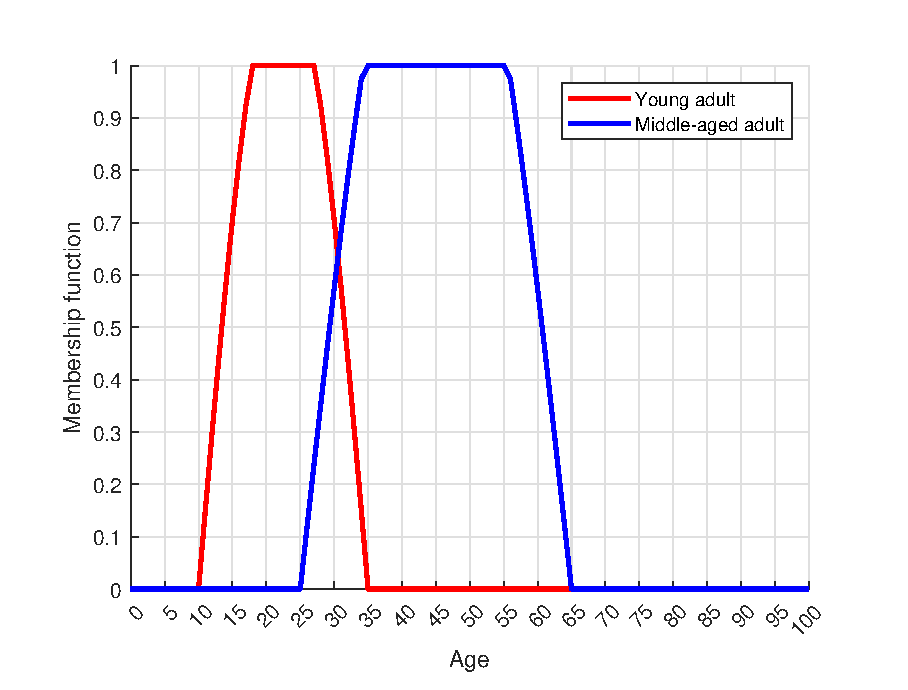
\includegraphics[width=250pt]{chapters/ch-fuzzy-control-system/figures/fuzzysetexp.eps}
	\caption{Membership function of fuzzy sets ``young adult'' and ``middle-aged adult''.} \label{ch:fcs:fig:fuzzysetexp}
\end{figure}

From Fig. \ref{ch:fcs:fig:fuzzysetexp}, we can see how a person is categorized according to the age. For example, a 5-year-old child is by no means a young adult or an adult, as $\mu_{A_1}=\mu_{A_2}(5)=0$ from the figure. A 15-year-old can be considered ``quite'' a young adult, with $\mu_{A_1}=0.7$.

The maximum value of a membership function is defined as the height of the fuzzy set. In many occasions the height is $1$, but it is not always the case. An element whose associated membership function equals to half of the height is called the crossover point.

It is possible to set up a threshold for the membership function, and derive a set from a fuzzy set as follows.
\begin{eqnarray}
	\utilde{A}_\alpha &=& \left\{e \middle| \mu_{\utilde{A}} (e) \geq \alpha \right\} \nonumber
\end{eqnarray}
Notice that $\utilde{A}_\alpha$ is a set (not a fuzzy set) of the original fuzzy set, known as the cut set. A fuzzy set can have infinite number of cut sets by choosing different $\alpha$. A fuzzy set can be derived from all its cut sets as follows.
\begin{eqnarray}
	\utilde{A} &=& \bigcup_{\alpha \in [0, 1]} \alpha A_\alpha \nonumber
\end{eqnarray}
where $\alpha A_\alpha$ is a fuzzy set defined on $ A_\alpha$ with constant membership function value $\alpha$.

Following the same concept, define the support and core of a fuzzy set as follows, respectively.
\begin{eqnarray}
	\textup{supp}(\utilde{A}) &=& \left\{ e \middle| \mu_{\utilde{A}}(e) > 0 \right\} \nonumber \\
	C(\utilde{A}) &=& \left\{ e \middle| \mu_{\utilde{A}}(e) = 1 \right\} \nonumber
\end{eqnarray}

A fuzzy set $\utilde{A}$ can be represented by its base set $A$ together with associated membership functions $\mu_{\utilde{A}}$. Alternatively, use the following
\begin{eqnarray}
	\utilde{A} &=& \sum_{i} \dfrac{\mu_{\utilde{A}}(e_i)}{e_i} \nonumber \\
	\utilde{A} &=& \int_{E} \dfrac{\mu_{\utilde{A}}(e)}{e} \nonumber
\end{eqnarray}
to represent a fuzzy set with discrete and continuous universe, respectively. Notice that in the above representation, ``$\cdot / \cdot$'' is not a division, and $\sum$, $\int$ are not summation and integration (although there are some connections), but just a conventional notation used in the fuzzy set.

\subsection{Fuzzy Set Operations}

Operations such as union and intersection are defined on fuzzy sets. They are summarized in Table \ref{ch:fcs:tab:fuzzysetoperation}.

\begin{table}[h]
	\centering
	\begin{tabular}{lll}
		\hline
		Operation & Symbol & Membership Function \\
		\hline
		Union & $\utilde{A} \cup \utilde{B}$ & $\mu_{\utilde{A} \cup \utilde{B}}(e) = \max(\mu_{\utilde{A}}(e), \mu_{\utilde{B}}(e))$ \\
		Intersection & $\utilde{A} \cap \utilde{B}$ & $\mu_{\utilde{A} \cap \utilde{B}}(e) = \min(\mu_{\utilde{A}}(e), \mu_{\utilde{B}}(e))$ \\
		Complement & $\utilde{A}'$ & $\mu_{\utilde{A}'}(e) = 1 - \mu_{\utilde{A}}(e)$ \\
		\hline
	\end{tabular}
	\caption{Commonly used fuzzy set operations.}
	\label{ch:fcs:tab:fuzzysetoperation}
\end{table}

Notice that Table \ref{ch:fcs:tab:fuzzysetoperation} gives only one out of many ways to define these operations. There are other ways to define them. For example, for complement, there is Sugeno's complement and Yager's complement as follows. The ones given in Table \ref{ch:fcs:tab:fuzzysetoperation} is the most commonly used definition.
\begin{eqnarray}
	N_s(e) &=& \dfrac{1-e}{1+\lambda e} \nonumber \\
	N_w(e) &=& (1-a^w)^{\frac{1}{w}} \nonumber
\end{eqnarray}

More operations can be found in \cite{mizumoto1981fuzzy}.

\subsection{Commonly Used Membership Functions}

Membership functions can be chosen flexibly as long as it is bounded by $[0, 1]$ for each element. There are some commonly used ones that has been proved useful in general problems as shown in Fig. \ref{ch:fcs:fig:commonmf}. They, together with their combinations, are widely used in fuzzy control system design.

\begin{figure}
	\centering
	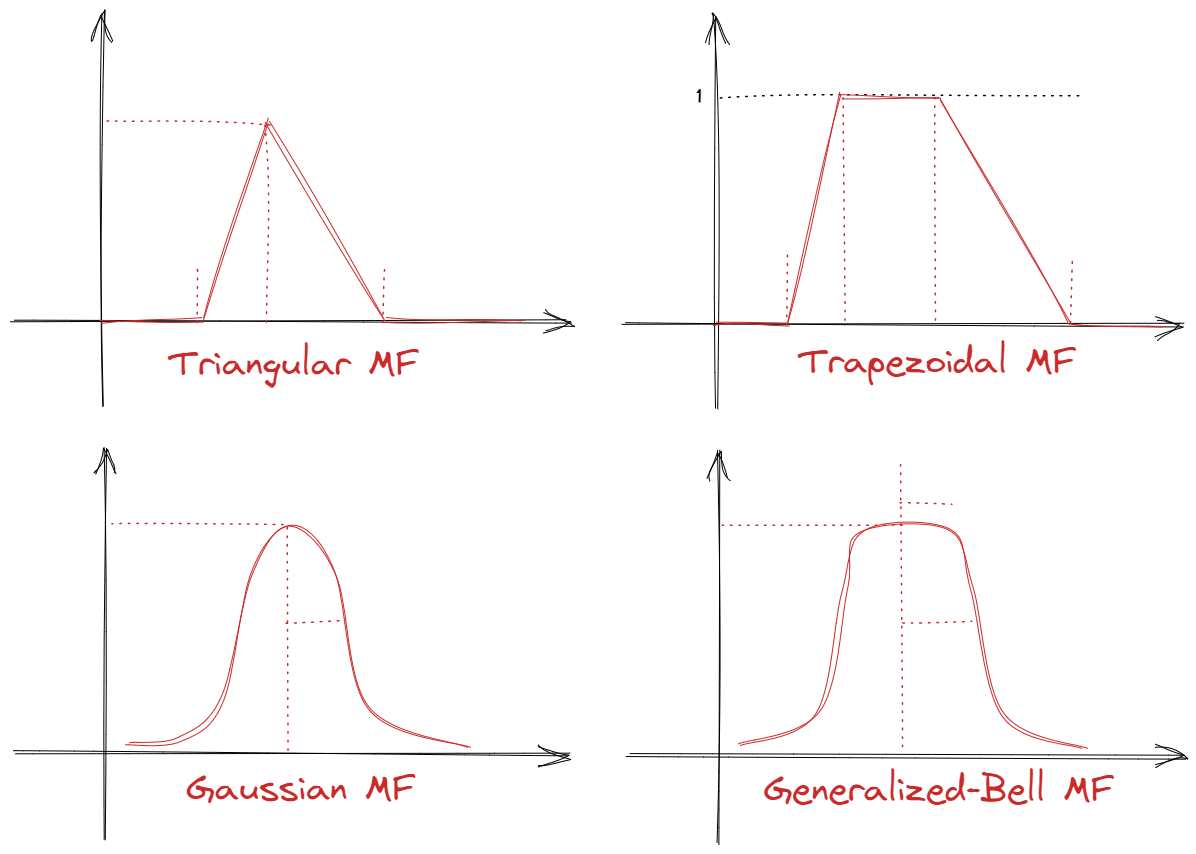
\includegraphics[width=350pt]{chapters/ch-fuzzy-control-system/figures/commonmf.png}
	\caption{Commonly used membership functions.} \label{ch:fcs:fig:commonmf}
\end{figure}

MATLAB provides built in functions to generate the functions in \ref{ch:fcs:fig:commonmf}, such as \verb|trimf| for triangular membership function, \verb|trapmf| for trapezoidal function, \verb|gaussmf| for Gaussian, and \verb|gbellmf| for generalized-bell function, respectively. There are other membership functions built-in to MATLAB as well.

\subsection{Fuzzy Relation}

In set theory, a relation of two elements is defined using sets. For example, let $a, b \in \mathbb{R}$. Let a customized relation ``$\oplus$'' be defined on $\mathbb{R} \times \mathbb{R} = \mathbb{R}^2$. We can say $a \oplus b$ if and only if there is a set defined on $\mathbb{R}^2$ associated with ``$\oplus$'' relation, and $(a,b)$ is in that set. Here ``$\times$'' denotes the Cartesian product.

Fuzzy relation is defined likewise, except that the set is replaced with fuzzy set as follows. Let $u\in U$, $v \in V$ be two variables with the same or different domains, and $D=U \times V$. The fuzzy relation of ``$\oplus$'' of two elements $u$ and $v$ is defined by the following fuzzy set
\begin{eqnarray}
	\mu_{\utilde{D}} (u,v) &\in& [0, 1] \nonumber
\end{eqnarray}
associated with ``$\oplus$''.

It is possible to use a matrix to record the fuzzy relations, in which case the matrix is called a fuzzy matrix as it is made up of membership functions. Other choice include fuzzy graph, which takes advantage of graph theory to represent the fuzzy relation of different nodes in a universe.

The relation can be derived from chains. For example, consider relation $P$ defined one $X \times Y$, and $Q$ on $Y \times Z$. A relation on $X, Z$ can be derived. One way (this is not the only way) is to use
\begin{eqnarray}
	\mu_{X \times Z}(x, z) &=& \sup \left[\min\left(\mu_{X\times Y}(x, y), \mu_{Y\times Z} (y, z)\right)\right] \nonumber
\end{eqnarray}

\section{Fuzzy Control System}

Fuzzy control system is a practice of utilizing fuzzy logics in engineering. It mainly includes fuzzification of the system, fuzzy interface, and fuzzy control system design. Details are covered in the remaining of this section.

\subsection{Basic Concepts}

A proposition refers to a mathematical statement, either being true or false. For example, $0 \in \mathbb{Z}$ is a true statement as zero belongs to the integer set. As another example, give $x=5$, $x \geq 3$ is a true statement.

Fuzzy proposition refers to ``ambiguous'' statements, that it is not a proposition from a mathematical perspective as it cannot be told whether true or false. An example is ``$x$ is large''. Instead of true/false, a fuzzy proposition is described by $\beta \in [0, 1]$ that describes to what extent the statement is considered as true. In the aforementioned example, if we define ``large'' as a fuzzy set, then fuzzy proposition ``$x$ is large'' is to the extent of $\beta = \mu_{\textup{large}}(x)$ true.

A reasoning is often formulated by ``if <proposition 1> then <proposition 2>''. The reasoning indicates that if the first proposition is true, so is the second proposition. The reasoning itself is also a proposition, as $A \rightarrow B$ is equivalent to $\bar{A}\cup (A\cap B)$. Under the fuzzy logic scope, the propositions are fuzzy propositions. An example is ``if service quality is good, tips is high''. Apparently, ``good'' is defined as a fuzzy set.

A reasoning can be taken as a rule. Rules are the basic representations of knowledge base in fuzzy control system, where each rule can be taken as an input from the expert.

\subsection{Fuzzification}

xxx

\subsection{Fuzzy Interface}

xxx

\subsection{Fuzzy Controller Design}

xxx

\subsection{Fuzzy Controller Performance Analysis}

xxx

\section{Fuzzy Modeling and Fuzzy System Identification}

xxx

\section{Examples}

A motivating example is given to introduce the basic use of fuzzy logics calculations. Several examples are given consecutively to demonstrate how to use MATLAB fuzzy logic toolbox to build fuzzy controllers.

\subsection{Motivating: Calculate Tips in a Restaurant}

Consider the example given below.

\begin{shortbox}
\Boxhead{A Motivating Example}

The tips that a customer pays to the waiter/waitress in a restaurant depends on the quality of the food and the service. It often has a lower and upper bound of $5\%$ to $25\%$ of the bill. When the quality of both the food and the service is exceptional, the tips will more likely to be close to $25\%$, vise versa, as shown in Fig. \ref{ch:fcs:fig:expmotivating}.

There is no matrix that quantifies the quality of the food, nor the service. It is more about how the customer feels objectively. Neither is there a fixed guidance that maps them to the tips, i.e., some customers may take food and service equality important, while others may think one more significant than the other.

Try to describe tips as a function of food and service quality.

\end{shortbox}

\begin{figure}
	\centering
	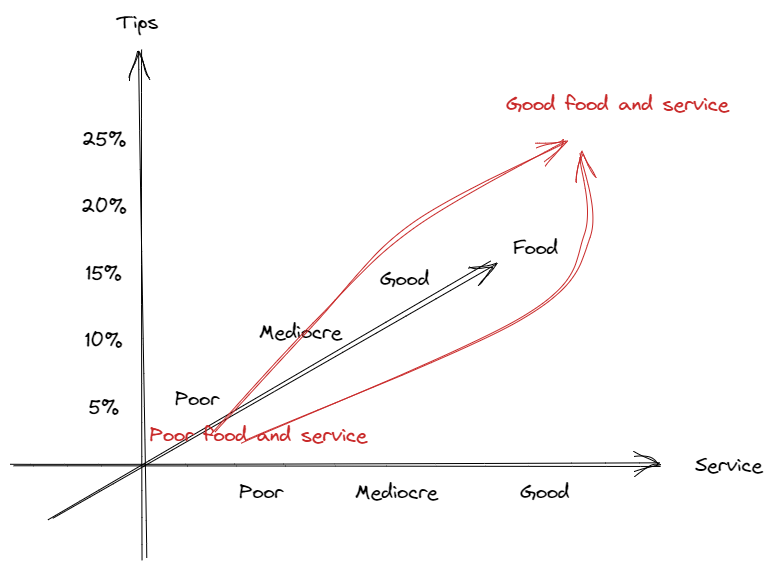
\includegraphics[width=250pt]{chapters/ch-fuzzy-control-system/figures/expmotivating.png}
	\caption{Tips relate to food and service quality.} \label{ch:fcs:fig:expmotivating}
\end{figure}

Solving the above problem using conventional methods requires precise modeling of how the customer's utility relates to food and service quality. An example is given below, where the utilities the customer gets from the service and food qualities modeled using an exponential function and a linear function, respectively. Finally, the tips are determined by a weighted sum of the utilities.
\begin{eqnarray}
	u_1 &=& \dfrac{e^{x_1}-1}{e-1} \nonumber \\
	u_2 &=& x_2 \nonumber \\
	u &=& 0.8 u_1 + 0.2 u_2 \nonumber \\
	\textup{tips} &=& (0.25-0.05)u + 0.05 \nonumber
\end{eqnarray}
where $x_1\in [0,1]$ and $x_2 \in [0,1]$ are used to characterize the service and food qualities, respectively. The result is given in plotted in Fig. \ref{ch:fcs:fig:motivatingexp_conventional}. It can be seen that although this is a common practical problem of daily life and a human can solve it almost immediately, the modeling and realization of the solution using conventional control method can be difficult. The conventional method, in this case, is non-intuitive and differs largely from how human would naturally handle this problem.

\begin{figure}
	\centering
	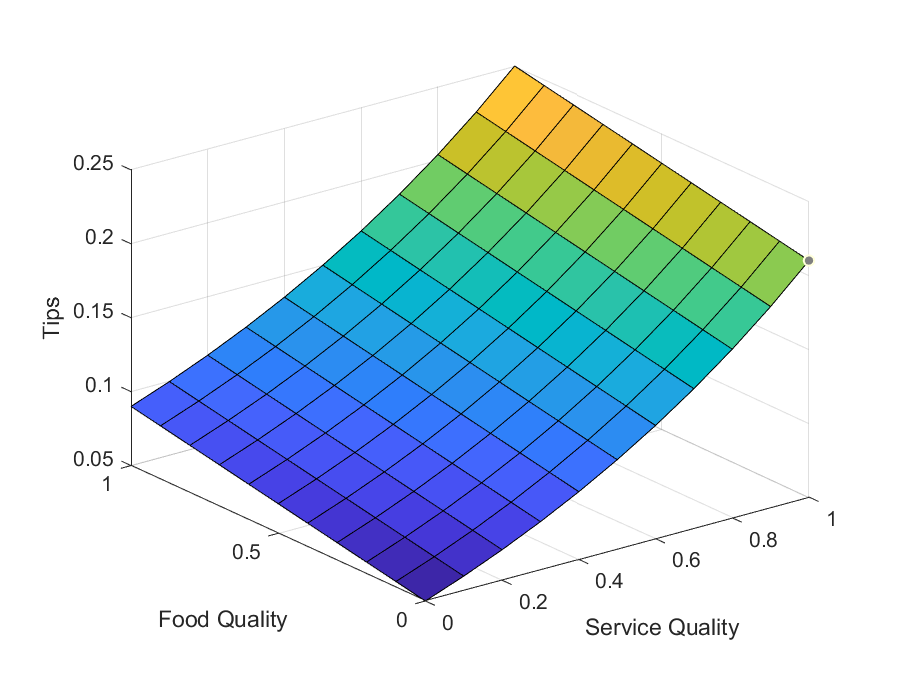
\includegraphics[width=250pt]{chapters/ch-fuzzy-control-system/figures/motivatingexp_conventional.eps}
	\caption{Tips as a deterministic function of service and food qualities.} \label{ch:fcs:fig:motivatingexp_conventional}
\end{figure}

MATLAB fuzzy control toolbox provides variety of tools to design and demonstrate fuzzy controllers. For the aforementioned problem, a built-in fuzzy interface system (FIS) named ``tipper'' is defined. A fuzzy inference is the process of formulating the mapping from a given input to an output using fuzzy logics. More details of FIS is introduced elsewhere in this chapter.

In tipper, 3 fizzy variables (2 inputs, 1 output) and 3 rules are defined. The result is plotted in Fig. \ref{ch:fcs:fig:motivatingexp_fis}. By comparing Figs. \ref{ch:fcs:fig:motivatingexp_conventional} and \ref{ch:fcs:fig:motivatingexp_fis}, it can be seen that fuzzy logics can interpret ``good service'', ``bad service'', etc., in a more intuitive way close to human, and it can formulate more complicated behavior with simpler setup. It requires rules instead of tons of samples (for training) to form this behavior.

\begin{figure}
	\centering
	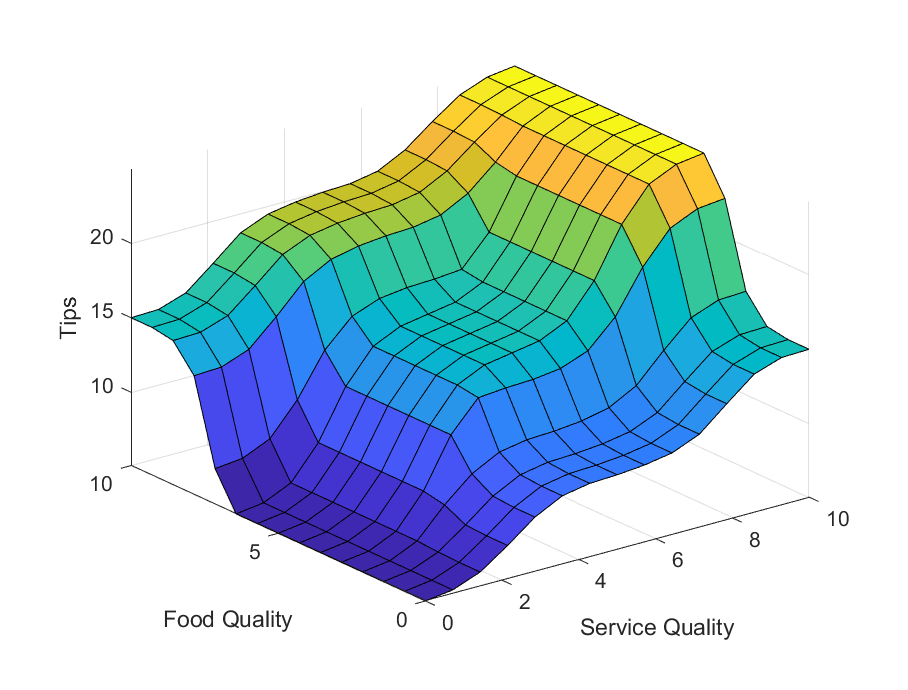
\includegraphics[width=250pt]{chapters/ch-fuzzy-control-system/figures/motivatingexp_fis.eps}
	\caption{Tips as a deterministic function of service and food qualities using fuzzy logic.} \label{ch:fcs:fig:motivatingexp_fis}
\end{figure}

\subsection{Defining Membership Functions for Fuzzy Sets}

Consider the following example.

\begin{shortbox}
	\Boxhead{Fuzzy Sets Creation}
	
	Define the following fuzzy sets in MATLAB. Let both $\utilde{A}$, $\utilde{B}$ be fuzzy sets with triangular membership function. Let $\utilde{C} = \utilde{A} + \utilde{B}$ whose elements are obtained by adding elements in $\utilde{A}$ and $\utilde{B}$.
	
\end{shortbox}

Create $\utilde{A}$ and $\utilde{B}$ as follows. Their membership function is plotted in Fig. \ref{ch:fcs:fig:exp_createfuzzyset} as the red and blue lines, respectively.
\begin{lstlisting}[style=Matlab-editor]
x = 0:0.01:10;
trimf_a = @(x) 0.9*trimf(x, [1, 2, 3]);
trimf_b = @(x) trimf(x, [2, 5, 6]);
a = trimf_a(x);
b = trimf_b(x);
\end{lstlisting}

\begin{figure}
	\centering
	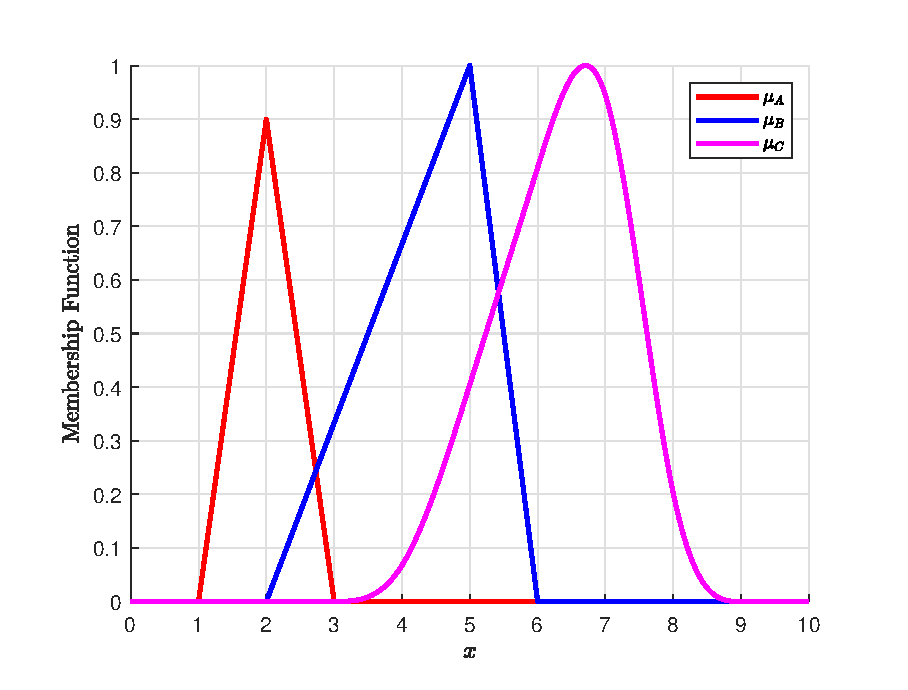
\includegraphics[width=250pt]{chapters/ch-fuzzy-control-system/figures/exp_createfuzzyset.eps}
	\caption{Create fuzzy sets membership functions for in MATLAB.}
	\label{ch:fcs:fig:exp_createfuzzyset}
\end{figure}

Variables in $\utilde{C}$ is obtained by adding elements in $\utilde{A}$ and $\utilde{B}$. For example, consider $c = 7$. This can be achieved from a set of combinations $a=0, b=7$, $a=0.01, b=6.99$, ..., $a = 7, b = 0$. The membership function, $\mu_{\utilde{C}(7)}$, is a sum of the membership function of all the combinations, where in each combination the associated membership function is obtained by multiplying (this is only one of the ways to handle this problem) the membership functions of $\utilde{A}$ and $\utilde{B}$. Finally, the membership function is normalized by dividing it with its maximum value.

Use the following to calculate the membership function of $\utilde{C}$ as illustrated above. The result is plotted in Fig. \ref{ch:fcs:fig:exp_createfuzzyset} as the magenta line
\begin{lstlisting}[style=Matlab-editor]
	c = conv(a, b, 'full');
	c = c(1:length(x));
	c = c/max(c);
\end{lstlisting}

\subsection{Fuzzy Approximation}

Fuzzy approximation tries to describe complicated functions using sets of  fuzzy rules.













